
\documentclass[12pt]{book}
 
\usepackage[margin=1in]{geometry} 
\usepackage{amsmath,amsthm,amssymb}
\usepackage{graphicx}
\usepackage{float}
\usepackage{blindtext}
\usepackage{pst-node}
\usepackage{pdfpages}
% \usetikzlibrary{shapes, positioning, arrows.meta}
% \usetikzlibrary{decorations, decorations.markings}
    % \usepackage{tikz}
    % \usetikzlibrary{graphs,graphdrawing,quotes}
    % \usegdlibrary{trees}

\usepackage{pst-plot}
\newcommand{\N}{\mathbb{N}}
\newcommand{\Z}{\mathbb{Z}}

\newenvironment{theorem}[2][Theorem]{\begin{trivlist}
\item[\hskip \labelsep {\bfseries #1}\hskip \labelsep {\bfseries #2.}]}{\end{trivlist}}
\newenvironment{lemma}[2][Lemma]{\begin{trivlist}
\item[\hskip \labelsep {\bfseries #1}\hskip \labelsep {\bfseries #2.}]}{\end{trivlist}}
\newenvironment{exercise}[2][Exercise]{\begin{trivlist}
\item[\hskip \labelsep {\bfseries #1}\hskip \labelsep {\bfseries #2.}]}{\end{trivlist}}
\newenvironment{problem}[2][Problem]{\begin{trivlist}
\item[\hskip \labelsep {\bfseries #1}\hskip \labelsep {\bfseries #2.}]}{\end{trivlist}}
\newenvironment{question}[2][Question]{\begin{trivlist}
\item[\hskip \labelsep {\bfseries #1}\hskip \labelsep {\bfseries #2.}]}{\end{trivlist}}
\newenvironment{corollary}[2][Corollary]{\begin{trivlist}
\item[\hskip \labelsep {\bfseries #1}\hskip \labelsep {\bfseries #2.}]}{\end{trivlist}}

\newenvironment{solution}{\begin{proof}[Solution]}{\end{proof}}

\begin{document}
 
% --------------------------------------------------------------
%                         Start here
% --------------------------------------------------------------
 
\title{Pricing Modeling Notes}%replace X with the appropriate number
\author{\\ %replace with your name
} %if necessary, replace with your course title
 
\maketitle
 
% \begin{theorem}{x.yz} %You can use theorem, exercise, problem, or question here.  Modify x.yz to be whatever number you are proving
% Delete this text and write theorem statement here.
% \end{theorem}
 
% \begin{proof} %You can also use solution in place of proof.
% Blah, blah, blah.  Here is an example of the \texttt{align} environment:
%Note 1: The * tells LaTeX not to number the lines.  If you remove the *, be sure to remove it below, too.
%Note 2: Inside the align environment, you do not want to use $-signs.  The reason for this is that this is already a math environment. This is why we have to include \text{} around any text inside the align environment.

\chapter{Loan Pricing}
\section{ Preliminary definitions} 
\subsection{Default and Prepayment probabilities:}
$ \forall t \in \{1,2,...T\}$
\[ % <-- step a
\begin{array}{rr} % <-- steps b and c
   p_p(t)  :&  \mbox{
   Probability that the loan will prepay at time t given that it has survived to that point } \\
   p_p(t)  : &  \mbox{
   Probability that the loan will default at time t given that it has survived to that point
   }
\end{array} \noindent% <-- step e
\] % <-- step e

 \subsection{Survival function:}
$S(t)$ :   Probability that a loan survives until period t 
\begin{align}
S(t) & = \Pi_{s=1}^t (1-p_d(s) - p_p(s)) \\
 & = (1-p_d(1) - p_p(1))\times(1-p_d(2) - p_p(2))\times...\times(1-p_d(t) - p_p(t)) \nonumber
\end{align}

\subsection{Balance function: }
The Current Balance function $\bar{B}(t)$ is the remaining balance left at time $t-1$ for a loan with principal $B=\bar{B}(1)$ and in absence of any prepayment or default risk. For non conventional loan payments this function might not have a closed form solution. 


\paragraph{Constant installments:} The remaining balance at time $t$ for a loan with principal (Balance at t=0) B is given by 
\begin{align}
\bar{ B}(t)&=B\frac{(1+r)^T-(1+r)^{t-1}}{(1+r)^T-1}
\end{align}
\begin{align}
\bar{ I}(t)&=r\times \bar{ B}(t)
\end{align}
The acute reader will notice that the definition of $\bar{ B}(t)$, in terms of the remaining balance left at time $t-1$ , was given so that we can state such a simple equation for $\bar{ I}(t)$.


\paragraph{Constant amortization: } The remaining balance at time $t$ for a loan with principal (Balance at t=0) B is given by:

\begin{align}
\bar{ B}(t)&=B \times (1-\frac{t-1}{T})
\end{align}


\section{ Terms included in the incremental profit (CLV)}
\subsection{ Interest on loans: }
\begin{align}
LI(t) = S(t)\bar{ B}(t)r
\end{align}
\subsection{  Cost of Funds: }
\begin{align}
COF(t) = S_c(t)\bar{ B}_c(t)r_c
\end{align}
Where: 
\begin{align}
S_c(t)= \Pi_{s=0}^t [1- p_p(s)-(1-LGD(s))p_d(s) ]
\end{align}

\subsection{ Equity Benefit (Captal Rebate): }
\begin{align}
EB(t) = \alpha S(t)\bar{ B}(t) r_c
\end{align}

\subsection{ Fees Additional Source of revenue: }
\begin{align}
F(t) = f S(t)
\end{align}

\subsection{ Servicing Costs: }
\begin{align}
SC(t) =  \sigma S(t)
\end{align}

\subsection{ Loss from Default: }
\begin{align}
EL(t) =  p_d(t)LGD(t)S(t)\bar{ B}(t) 
\end{align}
\subsection{Recovery costs}
\begin{align}
C(t) = c\times p_d(t) S(t)
\end{align}

\subsection{ Equity Capital Charge: }
\begin{align}
 EC(t) =  \alpha S(t)\bar{ B}(t) r_e
\end{align}


\section{ Incremental Profit Definition (CLV): }
The net present value is given by:

\begin{align}
NPV(x(t),r,T)=\sum_{t=1}^T \frac{x(t)}{(1+r)^t}
\end{align}

\renewcommand{\arraystretch}{1.5} % <-- optional a
\begin{center} % <-- optional b
\[ % <-- step a
\begin{array}{|l|c|l|} \hline % <-- steps b, c; optional c, d
\mbox{Element} & \mbox{Notation} & \mbox{Calculation}\\ \hline
\mbox{ Lending Interest }  & LI & NVP(LI(t),r_d,T)\\
\mbox{Cost of Funds   }  & COF & NVP(COF(t),r_d,T)\\
\mbox{Equity benefit }  & EB & NVP(EB(t),r_d,T)\\
\mbox{Fees }  & LI & NVP(F(t),r_d,T)\\
\mbox{ Ancillary profit }  & A & -\\
\mbox{Origination cost}  & OC & -\\
\mbox{ Commision  }  & COM & -\\
\mbox{ Servicing Costs}  & SC & NVP(SC(t),r_d,T)\\
\mbox{ Expected Loss }  & EL & NVP(EL(t),r_d,T)\\
\mbox{ Collection costs }  & C & NVP(C(t),r_d,T)\\
\mbox{ Equity charge}  & EC & NVP(EC(t),r_d,T)\\

\hline
\end{array} % <-- step e
\] % <-- step e
\end{center}

\renewcommand{\arraystretch}{1.5} % <-- optional a
\begin{center} % <-- optional b
\[ % <-- step a
\begin{array}{|l|c|l|} \hline % <-- steps b, c; optional c, d
\mbox{Element} & \mbox{Notation} & \mbox{Calculation}\\ \hline
\mbox{ Net Interest Income }  & NII & LI-COF+EB\\
\mbox{Total Income  }  & TI & NII+A+F\\
\mbox{Net Income before tax}  & NIBT & TI-OC-COM-SC-LD-C\\
\mbox{Net Income after tax }  & NIAT&(1-\tau)\times NIBT \\
\mbox{ Incremental profit  }  & IP & NIAT-EC\\

\hline
\end{array} % <-- step e
\] % <-- step e
\end{center}

\subsection{ Incremental Profit Function: }
Define the incremental profit function as:
\begin{align}
\pi(p)=IP(p)
\end{align}
%Page on setup equations
\section{Financial Math operators}
\subsection{Constant Installments}
We can define a $c_f$ factor to compute constant installments by defining the following:
\begin{align}
    B(1) &= \frac{c}{(1+r)}+\frac{c}{(1+r)^2}+\frac{c}{(1+r)^3}+...++\frac{c}{(1+r)^T} \nonumber\\
    &=c\delta[1+\delta+\delta^2+\delta^3+\delta^4+...+\delta^{T-1}] \nonumber \\
    &=c\delta\left[\frac{1}{1-\delta}-\delta^T\frac{1}{1-\delta}\right] =c\delta\left(\frac{1-\delta^T}{1-\delta}\right)
\end{align}
\begin{align}
    c=B(1)\left(\frac{1-\delta}{\delta}\right)\frac{1}{1-\delta^T}=B(1)\left[r\frac{(1+r)^T}{(1+r)^T-1}\right]
\end{align}

\begin{align}
    c_f(r,T):=\frac{r(1+r)^T}{(1+r)^T-1} \implies c:=B(1)c_f(r,T)
\end{align}

Balance factor:
\begin{align}
    B(t)=B(1)\left[ \frac{(1+r)^T-(1+r)^{t-1}}{(1+r)^T-1} \right]
\end{align}
\begin{align}
    B_f(t,r,T)=\left[ \frac{(1+r)^T-(1+r)^{t-1}}{(1+r)^T-1} \right] \implies B(t)=B(1)B_f(t,r,T)
\end{align}
\begin{align}
    \bar{I}(t) = rB(1)B_f(t,r,T)
\end{align}
Amortization factor:
\begin{align}
    A_f(t,r,T) &= c_f(r,T)-rB_f(t,r,T)\\
    &=\frac{r(1+r)^{t-1}}{(1+r)^T-1}
\end{align}


\begin{theorem}{1.1 (Telescopic amortizations)}{} Let
\[
\prod^{t-1}_{s=1}(1-A(1,r,T-s+1))=1-\sum^{t-1}_{s=1}A(s,r,T)
\]
\end{theorem}

\begin{proof}{}{} Lets define
\[
E_1=\prod^{t-1}_{s=1}(1-A(1,r,T-s+1)), \\
E_2 =1-\sum^{t-1}_{s=1}A(s,r,T)
\]
and
\[
\delta =1/(1+r)
\]


\end{proof}

%  Page on setup examples
\section{Alternative sequences for computing Incremental Profit}



\subsection{Canonical model}
\begin{figure}[H]
  \centering
      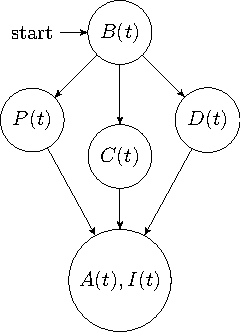
\includegraphics[width=.3\textwidth]{Graph2.pdf} 
 \caption{Graph for computations}
 \label{fig:graph2}
\end{figure}

\begin{center} % <-- optional b
\[ % <-- step a
\begin{array}{|l|c|l|} \hline % <-- steps b, c; optional c, d
\mbox{Variable} &\mbox{Notation} & \mbox{Calculation}\\ \hline
\mbox{Balance in presence of risk }  & B(t)  & B(t)\\
\mbox{Default  }  & D(t) & p_d(t) B(t)\\
\mbox{Full Prepayment}  & C(t) & p_c(t) B(t)\\
\mbox{Prepayment  }  & P(t) & p_p(t)B(t)\\
\mbox{Amortization}  & A(t) &(1-p_d(t)-p_c(t)-p_p(t)) B(t)A_f(1,r,T))\\
\mbox{Interest }  & \bar{I}(t) & (1-p_d(t)-p_c(t)-p_p(t))(1-A_f(1,r,T))B(t)r\\
\mbox{Principal   }  &  B(1) & B\\
\hline
\end{array} % <-- step e
\] % <-- step e
\end{center}
\pagebreak







\subsection{Prepayment dependent on initial balance}
\begin{figure}[H]
  \centering
      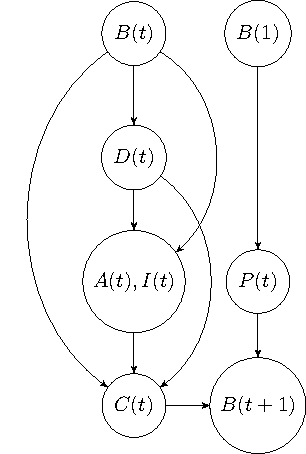
\includegraphics[width=.3\textwidth]{Graph1.pdf} 
 \caption{Topological Sort for computations}
 \label{fig:Test}
\end{figure}

\begin{center} % <-- optional b
\[ % <-- step a
\begin{array}{|l|c|l|} \hline % <-- steps b, c; optional c, d
\mbox{Variable} &\mbox{Notation} & \mbox{Calculation}\\ \hline
\mbox{Balance in presence of risk }  & B(t)  & B(t)\\
\mbox{Default  }  & D(t) & (1-p_d(t)) B(t)\\
\mbox{Amortization}  & A(t) &(1-p_d(t)) B(t)A(1,r,T))\\
\mbox{Interest }  & \bar{ I}(t) & (1-p_d(t))B(t)r\\
\mbox{Full Prepayment}  & C(1) & p_c(t) B(t)[1-p_d(t)-(1-p_d(t))A(1,r,T)]\\
\mbox{Principal   }  &  B(1) & B\\
\mbox{Prepayment  }  & P(t) & p_d(t)B\\
\hline
\end{array} % <-- step e
\] % <-- step e
\end{center}
\pagebreak
Notice that we defined $B(t)$ as the Loan Balance subject to risk (Conductual affected Loan Balance), as opposed to $\bar{B}(t)$, which is the Risk Free Loan Balance (Contractual Balance).  Given this definitions we can compute the recursive form for the balance function $B(t)$
\begin{align}
\scriptstyle
     \bar{B}(t+1) =&\scriptstyle \bar{B}(t)[1-p_d(t)-p_c(t)(1-p_d(t)-(1-p_d(t))A(1,r,T))-(1-p_d(t))A(1,r,T) ]-p_p(t) \bar{B}(1) \nonumber\\
    =&\scriptstyle \bar{B}(t)[1-p_d(t)-p_c(t)+p_d(t)p_c(t)+p_c(t)(1-p_d(t)A(1,r,T)-(1-p_d(t))A(1,r,T)]
    -p_p(t) \bar{B}(1) \nonumber\\
    =&\scriptstyle
    \bar{B}(t)[ (1-p_d(t))(1-p_c(t))-(1-p_d(t))(1-p_c(t))A(1,r,T)]
    -p_p(t) \bar{B}(1) \nonumber\\
     =&\scriptstyle
    \bar{B}(t)(1-p_d(t))(1-p_c(t))(1-A(1,r,T))
    -p_p(t) \bar{B}(1) \label{eq:bbar}\
\end{align}
Notice that (\ref{eq:bbar}) is a first order equation in difference which can be easily solved as.
\begin{align}
    \bar{B}(t) =\prod^{t-1}_{s=1} (1-A(1,r,T-s+1))(1-p_d(t))(1-p_p(t))B-\sum (\prod a_s) b_k
\end{align}
Using theorem () we can state the conductual balance$B(t)$ as a function of the contractual balance.



\section{Willingness to Pay (WTP): }
\subsection{The Price-Response Function}
Each price-response function specifies the demand that the lender would experience at each pricie, which will depend on:
\begin{enumerate}
    \item Total number of clientes interested in the loan
    \item Number of applicant clients
    \item The number of applicat the lender deems creditworthy and quotes a price.
    \item Number of accepted applicants who would achieve a positive surplus from taking the loan from the lender at the offered price.
    \item Number of accepted applicants who \textbf{ take up} the offered loan.
\end{enumerate}
In most lending markets, the final price is not known to the client at the time she applies for the loan so we assume that the number of clients who apply for a loan is not influenced by the price.
\begin{align}
d(p)=D\bar{F}(p)
\end{align}
$d(p)$ is the number of the loans offered by a lender that would be taken up at the price p. $D$ is the number of successful applicants for the loan, and $\overline{F}(p)$ is the take-up rate, which is defined as the fraction of successful applicants who will take up the loan at price $p$
\begin{align}
d(p)=D\bar{F}(p)
\end{align}
\begin{align}
\bar{F}(p)=\int^\infty_p f(w)dw
\end{align}
\subsection{Segmented vs Join Estimation}
For $n$ segments, the segmented estimation assumes each segments has its own demand function so we need to estimate $2n$ parameters.
\begin{align}
\bar{F_i}(p_i)=\frac{e^{a_i+b_i p_i}}{1+e^{a_i+b_i p_i}}
\end{align}

For $n$ segments, the join estimation assume we can estimate one single price price response function that includes all explanatory variables within it (including price)
\begin{align}
\bar{F}(p_i,a,b,\theta,x_i)=\frac{e^{a+b p_i+\theta^T x_i}}{1+e^{a+b p_i+\theta^T x_i}}
\end{align}

\section{Price optimization (CLV+WTP): }
\subsection{Price optimization without constraints}
\begin{align}
p^*= \arg \max_p \sum_{i=1}^N D_i\overline{F}_i(p_i)\pi(p)
\end{align}

\subsection{Price optimization with competing objectives: The efficient Frontier}

\begin{align}
p^*_j= \arg \max_p \sum_{i=1}^N D_i\bar{F}_i(p_i)\pi(p)
\end{align}
\begin{center}
    $s.t.$
\end{center}
\begin{align}
\sum_{i=1}^N D_i\bar{F}_i(p_i) =q_j,& \forall j
\end{align}


\chapter{Survival models}
\subsection{Common survival setup}
Let T be a positive random variable in $1,2,3,...$
\begin{align}
    S(t)=&P(T>t) \\
    F(t)=&1-S(t)=1-P(T>t)=P(T\leq t)
\end{align}
\subsection{Survival setup in presence of competing risks}

We define the cumulative incidence function as:
\begin{align}
    CIF_k(t)=&P(T\leq t,D=k) \\
    &=\sum_k P(T \leq t,D=k) = P(T \leq t)
\end{align}
In order to see what is the relationship between the CIF function and the usual conditional probability of default (death) we state the definition of conditional probability and use the fact that the event $T=t+1 \wedge T>t$ is equal to $T=t+1$ standalone.
\begin{align}
    p_k(t+1)&=p(T=t+1,D=k/T>t)=\frac{P(T=t+1,D=k)}{P(T>t)}\\
    &= \frac{ P(T \leq t+1,D=k)-P(T\leq t,D=k)}{
    1-\sum_k P(T \leq t, D=k)
    }
\end{align}

As an example lets consider that $D=1$ represents default
and $D=2$ represents prepayment then the conditional probabilities of default and prepayment are given by:
\begin{align}
p_d(t+1)&= \frac{CIF_d(t+1)-CIF_d(t)  }{
1- CIF_d(t)-CIF_p(t)}  
\end{align}

% --------------------------------------------------------------
%     You don't have to mess with anything below this line.
% --------------------------------------------------------------

 
\end{document}